\documentclass[12pt]{amsart}
%\usepackage{geometry}
%\geometry{
%	letterpaper,
%	total={8.5in,11in},
%	left=25mm,
%	right=25mm, 
%	top=5mm,
%	bottom=13mm,
%}

% Package Being Used:
\usepackage{amsmath}
\usepackage{amssymb}
\usepackage{bm}
\usepackage{graphicx}
\usepackage{psfrag}
\usepackage{color}
\usepackage{hyperref}
\hypersetup{colorlinks=true, linkcolor=blue, citecolor=magenta, urlcolor=violet}
\usepackage{url}
\usepackage{algpseudocode}


\usepackage{fancyhdr}
\usepackage{mathtools}
\usepackage{tikz-cd}
\usepackage{xy}
\input xy
\xyoption{all}
\usepackage{stmaryrd}
\usepackage{calrsfs}


% Paper Format and Geometry:
\voffset=-1.4mm
\oddsidemargin=10pt
\evensidemargin=10pt
\topmargin=0pt
\headheight=9pt     
\textheight=576pt
\textwidth=441pt
\parskip=0pt plus 4pt

\usepackage{fancyhdr}
\fancypagestyle{plain}{
	\fancyhf{} %Clear Everything.
%	\fancyfoot[C]{\thepage} %Page Number
	\renewcommand{\headrulewidth}{1pt} %0pt for no rule, 2pt thicker etc...
	\renewcommand{\footrulewidth}{0pt}
%	\fancyfoot[L]{BOTTOM LEFT}
%	\fancyfoot[R]{BOTTOM RIGHT}
	\fancyhead[L]{\fontsize{12}{12}\selectfont \textbf{Marcos Tirador}}
	\fancyhead[R]{\fontsize{11}{11}\selectfont Curriculum Vitae}
	\fancyfoot[LE,RO]{\thepage}
%	\fancyhead[RO]{TOP RIGHT, ODD PAGES}
}

\pagestyle{plain}
% Head Labels:
%\fancyhf{}
%\renewcommand{\headrulewidth}{1pt} 	 	
%\renewcommand{\footrulewidth}{0pt}
%\fancyhead[CE]{\fontsize{10}{11}\selectfont \textbf{Marcos Tirador} \hfill Curriculum Vitae}
%\fancyhead[CO]{\fontsize{10}{11}\selectfont \textbf{Marcos Tirador} \hfill Curriculum Vitae}
%\fancyhead[CO]{\fontsize{9}{11}\selectfont ON THE ATOMICITY OF POWER MONOIDS OF PUISEUX MONOIDS}
%\fancyhead[LE,RO]{\thepage}
%\setlength{\headheight}{9pt}


% Theorems-like Format and Numbering:
\newtheorem*{maintheorem*}{Main Theorem}
\newtheorem{theorem}{Theorem}[section]
\newtheorem{prop}[theorem]{Proposition}
\newtheorem{conj}[theorem]{Conjecture}
\newtheorem{lem}[theorem]{Lemma}
\newtheorem{cor}[theorem]{Corollary}
\theoremstyle{definition}
\newtheorem{defn}[theorem]{Definition}
\newtheorem{rem}[theorem]{Remark}
\newtheorem{example}[theorem]{Example}
\newtheorem{prob}[theorem]{Problem}
\newtheorem{question}[theorem]{Question}
\numberwithin{equation}{section}


% Personalized Commands:
\newcommand{\cc}{\mathbb{C}}
\newcommand{\ff}{\mathbb{F}}
\newcommand{\nn}{\mathbb{N}}
\newcommand{\pp}{\mathbb{P}}
\newcommand{\ppp}{\mathcal{P}}
\newcommand{\qq}{\mathbb{Q}}
\newcommand{\rr}{\mathbb{R}}
\newcommand{\zz}{\mathbb{Z}}
\newcommand{\ch}{\text{char}}
\newcommand{\lcm}{\text{lcm}}
\providecommand\ldb{\llbracket}
\providecommand\rdb{\rrbracket}
\newcommand\pval{\mathsf{v}_p}
\newcommand{\gp}{\text{gp}}
\newcommand{\qf}{\text{qf}}
\newcommand{\supp}{\textsf{supp}}
\newcommand{\ii}{\mathcal{Irr}}
\newcommand{\uu}{\mathcal{U}}
\newcommand{\ppf}{\mathcal{P}_{\text{fin}}}
\newcommand{\ppx}{\mathcal{P}_{\text{fin}, 0}}
\newcommand{\inter}{\mathsf{int}}
\newcommand{\cone}{\mathsf{cone}}
\newcommand{\norm}[1]{\left\lVert#1\right\rVert}

\newcommand{\at}{\mathcal{A}}
\newcommand{\lf}{\lfoloor}
\newcommand{\fl}[1]{\lfloor#1\rfloor}
\newcommand{\cl}[1]{\lceil #1\rceil}
\newcommand{\ds}{\displaystyle}

%\keywords{Minkowski sum, power monoid, Puiseux monoid, atomicity, factorization theory}

%\subjclass[2010]{Primary: 13C05, 13A15, 13C13; Secondary: 13A15}

%para las entradas tabulares fancies
%\usepackage{scrlayer-scrpage} % Provides headers and footers configuration
\usepackage{titlesec} % Allows creating custom \section's
\usepackage{marvosym} % Allows the use of symbols
\usepackage{tabularx,colortbl} % Advanced table configurations
\usepackage{ebgaramond} % Use the EB Garamond font
\usepackage{microtype} % To enable letterspacing
\titleformat{\section}{\large\scshape\raggedright}{}{0em}{}[\titlerule] % Section formatting
\newcommand{\gray}{\rowcolor[gray]{.90}} % Custom highlighting for the work experience and

\begin{document}
	
%	\mbox{}
%	\title{On the atomicity of power monoids of Puiseux monoids}
	
	
%	\author{Victor Gonzalez}
%	\address{Department of Mathematics\\Miami Dade College\\Miami, FL 33135, USA}
%	\email{victorm.gonzalez0202@gmail.com}
%	
%	\author{Henrick Rabinovitz}
%	\address{Melrose School\\Melrose, MA 02176, USA}
%	\email{hrey77@gmail.com}
%	
%	\author{Pedro Rodriguez}
%	\address{School of Mathematics and Statistics\\Clemson University\\Clemson, SC 29634}
%	\email{pedror@clemson.edu}
	
%	\author{Marcos Tirador}
%	\address{Matcom, Universidad de La Habana, Habana 10400, Cuba}
%	\email{marcosmath44@gmail.com}
		

\date{\today}

	

\section{Contact Information}
\begin{minipage}[t]{0.65\textwidth} % Ajusta el ancho de la minipágina para tu info de contacto
	\vspace{0pt} % Alinea la parte superior de ambas minipáginas

	\textit{Full name:} Marcos Manuel Tirador Del Riego
	%	\vspace{-0.4cm}
	
	\textit{Email address:} marcosmath44@gmail.com
	%	\vspace{-0.4cm}
	
	\textit{Website:} \href{marcostirador.github.io}{marcostirador.github.io}
	
	\textit{GitHub:} \href{https://github.com/MarcosTirador}{Marcos Tirador - GitHub}
	
	\textit{LinkedIn:} \href{https://www.linkedin.com/in/marcos-tirador-3601502b7/}{Marcos Tirador - LinkedIn}
%	\vspace{0.5cm}
\end{minipage}%
\hfill % Espacio entre Cminipáginas
\begin{minipage}[t]{0.3\textwidth} % Ajusta el ancho de la minipágina para la foto
	\vspace{0pt} % Alinea la parte superior de ambas minipáginas
	\flushright % Alinea la foto a la derecha
	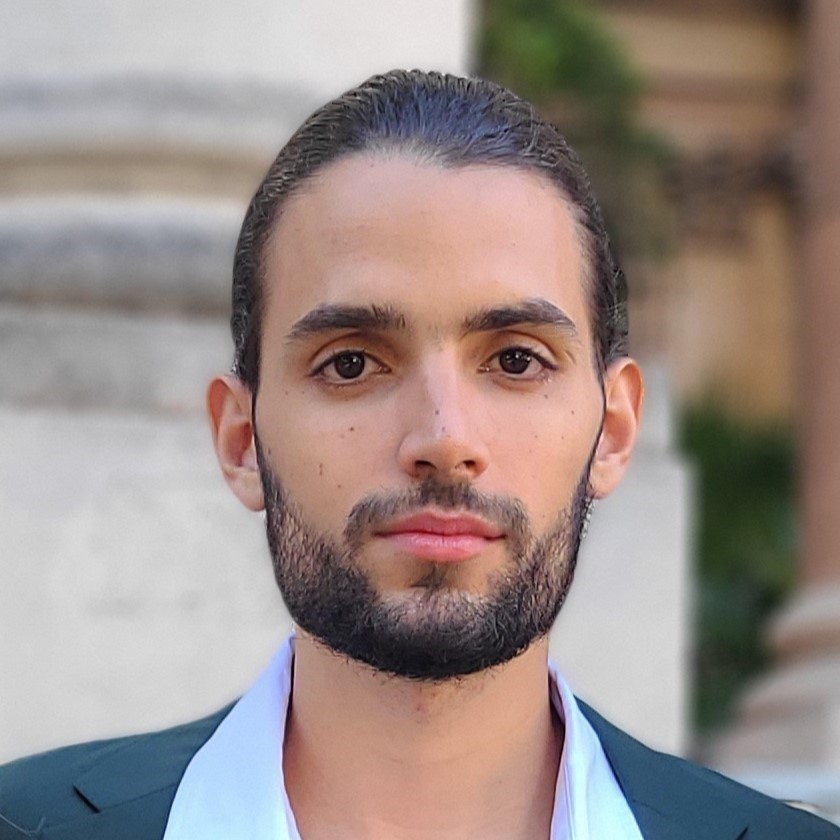
\includegraphics[width=70pt]{face5.jpg} % Asegúrate de ajustar la ruta a tu foto
\end{minipage}


	
\section{Summary}
Over the past four years, I have been conducting research in Mathematics and Computer Science, under the guidance of good mentors as the renowned Dr. Felix Gotti. A testament of my dedication, competitiveness, and problem-solving skills has been my participation in various contests, counting among my achievements having been a World Finalist in the ICPC. My primary interests lie in abstract algebra, artificial intelligence, blockchain technology, and theoretical computing. 

I also have expertise in various programming languages and technologies. Software development, in particular, appeals to me due to its creative process and the collaborative effort it entails. I love building solutions from the ground up, troubleshooting, and optimizing.

I am eager to explore opportunities where I can contribute to cutting-edge projects. I am particularly drawn to roles that challenge me to think outside the box and work alongside like-minded individuals passionate about making a tangible impact through technology.
 
%Within computer science my preference is for theoretical computing, but I have also developed good practical skills. In general I love to tackle complex problems that require creative thinking. These skills ICPC, where I am a World Finalist. 

%Within computer science my preference is theoretical computing. In general I love to tackle complex problems that require creative thinking. Problems of this type are often encountered in the ICPC, in which I am a World Finalist.

	
	
\section{Education}

	\begin{tabularx}{0.97\linewidth}{>{\raggedleft\scshape}p{2cm}X}
	\gray Period & \textbf{September 2019 --- January 2024}\\
	\gray Degree & \textbf{Bachelor of Science in Computer Science}\\
	\gray Rank & \textbf{Top of the class, golden diploma, outstanding  in research and academics}\\
	\gray University & \textbf{University of Havana} \hfill Havana, Cuba\\
	%& Extra information about degree
	\end{tabularx}
	
	\vspace{12pt}
	
	\begin{tabularx}{0.97\linewidth}{>{\raggedleft\scshape}p{2cm}X}
	\gray Period & \textbf{September 2015 --- May 2018}\\
	\gray Degree & \textbf{High School Diploma}\\
	%\gray Rank & \textbf{With Distinction}\\
	\gray School & \textbf{Vocational Pre-University Insitute of Exact Sciences Vladimir I. Lenin} \hfill Havana, Cuba\\
	%& Extra information about degree
	\end{tabularx}

\section{Work Experience}

		\begin{tabularx}{0.97\linewidth}{>{\raggedleft\scshape}p{2cm}X}
		\gray Period & \textbf{January 2024 --- Present Day}\\
		\gray Employer & \textbf{Department of Mathematics and Computer Science}\\
		\gray Job Title & \textbf{Researcher and instructor}\\
		\gray University & \textbf{University of Havana} \hfill Havana, Cuba\\
		%& Extra information about degree
	\end{tabularx}
%
%		\vspace{12pt}
%		
%		
%	\begin{tabularx}{0.97\linewidth}{>{\raggedleft\scshape}p{2cm}X}
%		\gray Period & \textbf{February 2022 --- July 2022}\\
%%		\gray Employer & \textbf{Department of Mathematics and Computer Science}\\
%		\gray Job Title & \textbf{Fullstack junior developer}\\
%		\gray Employer & \textbf{D' Clase (private tutoring company)} \hfill Havana, Cuba\\
%		%& Extra information about degree
%	\end{tabularx}
		
		\vspace{12pt}

	\section{Scientific Publications}
	
	\begin{enumerate}
		\item	\textit{On the set of molecules of numerical and puiseux monoids} \\(with Marly Gotti)\\ In: Rings, Monoids and Module Theory, Springer Proceedings in Mathematics \& Statistics book series (Eds. A. Badawi and J.
		Coykendall). Springer, Singapore. Vol. 382 (2022) 111–125, \href{https://doi.org/10.1007/978-981-16-8422-7_5}{doi:10.1007/978-981-16-8422-7\_5}.
		
		\item \textit{Factorization in additive monoids of evaluation polynomial semirings} \\ (with K. Ajran, J. Bringas, Bangzheng Li \& E. Singer) \\ Communications in Algebra, Vol. 51:10 (2023) 4347-4362, \href{https://doi.org/10.1080/00927872.2023.2208672}{doi:10.1080/00927872.2023.2208672}. 
		
		\item \textit{Subatomicity in Rank-2 Lattice Monoids} \\(with C. Liu \& P. Rodriguez)\\ Journal of Commutative Algebra (to appear). Preprint on \href{https://arxiv.org/abs/2308.01459}{ArXiv}. 
		
%		\item \textit{On the atomicity of power monoids of Puiseux monoids} \\(with V. Gonzalez , E. Li, H. Rabinovitz \& P. Rodriguez)\\ Submitted to International Journal of Algebra and Computations. Preprint on \href{https://arxiv.org/abs/2308.01459}{ArXiv}. 
	\end{enumerate}



\section{Awards}

	\begin{tabularx}{0.97\linewidth}{>{\raggedleft\scshape}p{2cm}X}
		\gray 2024 & \textbf{World Finalist at the International Collegiate Programming Contest (ICPC)}\\
	\end{tabularx}

	\begin{tabularx}{0.97\linewidth}{>{\raggedleft\scshape}p{2cm}X}
		\gray 2022 & \textbf{Bronze Medal at the XXV Iberoamerican University Mathematical Olympiad}\\
	\end{tabularx}
	
	\begin{tabularx}{0.97\linewidth}{>{\raggedleft\scshape}p{2cm}X}
		\gray 2022 & \textbf{Honorable Mention at the International Mathematics Competition
			for University Students}\\
	\end{tabularx}
		
	\begin{tabularx}{0.97\linewidth}{>{\raggedleft\scshape}p{2cm}X}
		\gray 2021 & \textbf{Bronze Medal at the International Mathematics Competition
			for University Students}\\
	\end{tabularx}
		
	\begin{tabularx}{0.97\linewidth}{>{\raggedleft\scshape}p{2cm}X}
		\gray 2021 & \textbf{Gold Medal at the Caribbean Finals of the International Collegiate Programming Contest (ICPC)}\\
	\end{tabularx}
	
	\begin{tabularx}{0.97\linewidth}{>{\raggedleft\scshape}p{2cm}X}
		\gray 2020 & \textbf{Bronze Medal at the Caribbean Finals of the International Collegiate Programming Contest (ICPC)}\\
	\end{tabularx}
	
	\begin{tabularx}{0.97\linewidth}{>{\raggedleft\scshape}p{2cm}X}
		\gray 2018 & \textbf{Bronze Medal at the Iberoamerican Mathematics Olympiad}\\
	\end{tabularx}
	
	\begin{tabularx}{0.97\linewidth}{>{\raggedleft\scshape}p{2cm}X}
		\gray 2017 & \textbf{Honorable Mention at the International Mathematical Olympiad (IMO)}\\
	\end{tabularx}
	
	\begin{tabularx}{0.97\linewidth}{>{\raggedleft\scshape}p{2cm}X}
		\gray 2016 & \textbf{Honorable Mention at the Central American and Caribbean Mathematics Olympiad}\\
	\end{tabularx}
	

\section{Teaching Experience}

	\begin{tabularx}{0.97\linewidth}{>{\raggedleft\scshape}p{2cm}X}
		\gray Period & \textbf{February 2024 --- Present Day}\\
		\gray Topic & \textbf{Introduction to Programming with Python}\\
		\gray Position & \textbf{Instructor}\\
		\gray Where & \textbf{Department of Mathematics and Computer Science} \hfill Havana, Cuba\\
	\end{tabularx}
	
	\vspace{12pt}

	\begin{tabularx}{0.97\linewidth}{>{\raggedleft\scshape}p{2cm}X}
		\gray Period & \textbf{February 2024 --- Present Day}\\
		\gray Topic & \textbf{Data Structures and Algorithms}\\
		\gray Position & \textbf{Instructor}\\
		\gray Where & \textbf{Department of Mathematics and Computer Science} \hfill Havana, Cuba\\
	\end{tabularx}

		\vspace{12pt}

	\begin{tabularx}{0.97\linewidth}{>{\raggedleft\scshape}p{2cm}X}
		\gray Period & \textbf{February 2022 --- January 2024}\\
		\gray Topic & \textbf{Data Structures and Algorithms}\\
		\gray Position & \textbf{Student Assistant}\\
		\gray Where & \textbf{Department of Mathematics and Computer Science} \hfill Havana, Cuba\\
	\end{tabularx}

	\vspace{12pt}
	
	\begin{tabularx}{0.97\linewidth}{>{\raggedleft\scshape}p{2cm}X}
		\gray Period & \textbf{May 2019 --- August 2019}\\
		\gray Topics & \textbf{Number Theory, Algebra and Combinatorics }\\
		\gray Position & \textbf{Math Instructor}\\
		\gray Where & \textbf{Cuban teams training for international competitions} \hfill Havana, Cuba\\
		%& Extra information about degree
	\end{tabularx}


\section{Technical Skills}
	\begin{tabular}{ @{} >{\bfseries}l @{\hspace{6ex}} l }
		Programming Languages & Python, C\#, C/C++, JavaScript, Haskell, Prolog, R \\ &(with a higher level of expertise in the first two) \\
		Developer Tools &  Git, Docker, Linux Systems \\
		Others & .NET Core, ASP.NET, React, SQL, Keras,
		\\&  spaCy, NTLK, scikit-learn, TensorFlow, 
	\end{tabular}
%	\textit{Programming languages:} 
%	\textit{Others:} 
%	\textit{Others:} 
		
\section{Soft Skills}

	Fast-learning, critical thinking, problem-solving, creativity, teamwork. 

\section{Language Skills}
	\begin{tabular}{ @{} >{\bfseries}l @{\hspace{6ex}} l }
	Spanish & Native Speaker \\
	English & Advanced (Certified by Doulingo English Test) 
\end{tabular}
%	\begin{itemize}
%		\item Spanish 
%	\end{itemize}	

%
\end{document}
\@setaddresses